\documentclass[tikz]{standalone}

\usepackage{tikz}
\usetikzlibrary{arrows.meta,positioning,fit,shapes.geometric,calc,decorations.pathreplacing,backgrounds}

\tikzset{
  >={Latex[length=2mm]},
  box/.style = {draw, rounded corners=2pt, align=center, minimum width=30mm, minimum height=8mm, thick, fill=white},
  group/.style = {draw, rounded corners=3pt, inner sep=6pt, thick, fill=gray!10},
  title/.style = {font=\bfseries\small, align=center, yshift=-1cm},
  line/.style = {thick},
  dot/.style = {circle, inner sep=1.9pt, draw=none, fill=gray!60},
  timeaxis/.style = {line width=1pt},
  timec/.style = {line width=0.5pt},
  timecActive/.style = {line width=1pt},
  flight/.style = {-{Latex[length=2.2mm]}, line width=1.5pt},
  flightFractional/.style = {-{Latex[length=2.2mm]}, line width=0.7pt},
  faint/.style = {draw=gray!50},
  dashedarrow/.style = {dash pattern=on 2.2pt off 2.2pt, -{Latex[length=2mm]}, line width=0.6pt, draw=gray!70},
  ghost/.style = {dash pattern=on 2.2pt off 2.2pt, draw=gray!60},
  attrLine/.style = {densely dashed, red, line width=1pt},
}

\newcommand{\groupBg}{
  \foreach \i in {0, \timeArcDy} {
    \draw[timeaxis, gray] (1,\i) -- (\xMax,\i);
  }
  \foreach \x in {1,...,\xMax} {
    \node[dot] (i\x) at (\x,0) {};
    \node[dot] (j\x) at (\x,\timeArcDy) {};
    \node[below=2pt of i\x] {\small $t_{\x}$};
  }
  \foreach \x in {1,...,\gpSize} {
    \draw[flight, gray!30, line width=0.5pt, dashed] (i\x) -- ($(i\x) + (\timeArcDx,\timeArcDy)$);
  }
}

\def\activeColor{blue}
\def\psgColor{orange}

\begin{document}
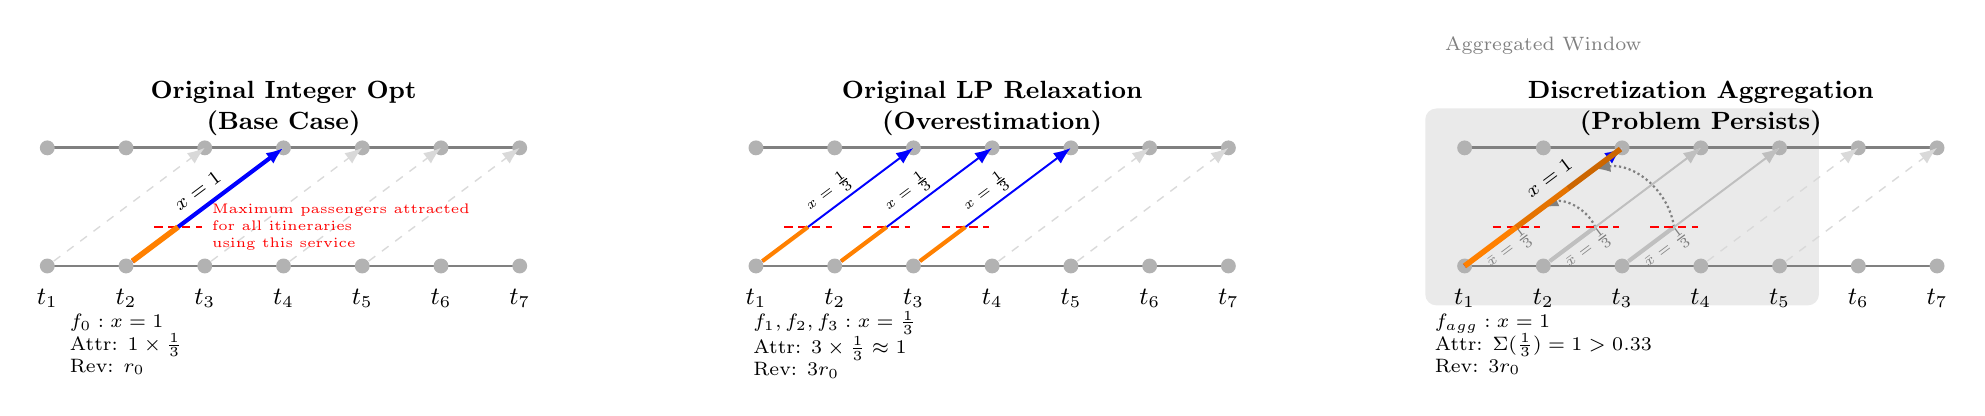
\begin{tikzpicture}
  % artificial padding
  % \draw [white] (-20,-10) rectangle (20,10);

  \def\gpSize{5}
  \def\timeArcDx{2}
  \def\timeArcDy{1.5}

  \pgfmathtruncatemacro{\xMax}{\gpSize + \timeArcDx}

  \def\psgMaxRatio{0.33} 
  
  % ----------------------------------------------------------------------
  % Case 1: Original Integer Optimal (Ground Truth)
  % ----------------------------------------------------------------------
  \begin{scope}[shift={(0,0)}]
    \node[title] at (\xMax/2+0.5, \timeArcDy + 1.5) {Original Integer Opt\\(Base Case)};
    \groupBg
    
    % One complete fleet assignment (f0) at t2
    \draw[flight, \activeColor] (i2) -- ($(i2) + (\timeArcDx,\timeArcDy)$) coordinate (dest2) node[midway, above, sloped, text=black] {\scriptsize $x=1$};
    
    % Attraction Max Line
    \draw[attrLine] (i2) ++(\psgMaxRatio*\timeArcDx - 0.3, \psgMaxRatio*\timeArcDy) -- ++(0.6, 0) node[right, font=\tiny, red, align=left] {Maximum passengers attracted\\for all itineraries\\using this service};

    % Orange revenue segment (only 0.33 attracted)
    \draw[line, \psgColor, line width=2pt] (i2) -- ($(i2) + (\psgMaxRatio*\timeArcDx,\psgMaxRatio*\timeArcDy)$);
    
    % Text
    \node[font=\scriptsize, align=left] at (2, -1) {
       $f_0: x=1$\\
       Attr: $1 \times \frac{1}{3}$\\
       Rev: $r_0$
    };
  \end{scope}

  % ----------------------------------------------------------------------
  % Case 2: Original LP Relaxation (Overestimation)
  % ----------------------------------------------------------------------
  \begin{scope}[shift={(9,0)}]
    \node[title] at (\xMax/2+0.5, \timeArcDy + 1.5) {Original LP Relaxation\\(Overestimation)};
    \groupBg
    
    % 3 fractional flights (f1, f2, f3) at t1, t2, t3
    \foreach \x in {1,2,3} {
        \draw[flightFractional, \activeColor] (i\x) -- ($(i\x) + (\timeArcDx,\timeArcDy)$) coordinate (dest\x) node[midway, above, sloped, text=black, yshift=-2pt] {\tiny $x=\frac{1}{3}$};

        % Attraction Max Line on Each (0.33)
        \draw[attrLine] (i\x) ++(\psgMaxRatio*\timeArcDx - 0.3, \psgMaxRatio*\timeArcDy) -- ++(0.6, 0);

        % Orange covers full effective length (which is visually 0.33 of the vector)
        \draw[line, \psgColor, line width=1.5pt] (i\x) -- ($(i\x) + (\psgMaxRatio*\timeArcDx,\psgMaxRatio*\timeArcDy)$);
    }
    
    % Text
    \node[font=\scriptsize, align=left] at (2, -1) {
       $f_1,f_2,f_3: x=\frac{1}{3}$\\
       Attr: $3 \times \frac{1}{3} \approx 1$\\
       Rev: $3r_0$
    };
  \end{scope}

  % ----------------------------------------------------------------------
  % Case 3: Discretization Aggregation (Persistence of Problem)
  % ----------------------------------------------------------------------
  \begin{scope}[shift={(18,0)}]
    \node[title] at (\xMax/2+0.5, \timeArcDy + 1.5) {Discretization Aggregation\\(Problem Persists)};
    
    % 1. Rect
    \begin{scope}[on background layer]
        \fill[gray!20, opacity=0.8, rounded corners] (0.5, -0.5) rectangle (3.5 + \timeArcDx, \timeArcDy + 0.5);
    \end{scope}
    \node[gray, font=\scriptsize] at (2, 2.8) {Aggregated Window};

    \groupBg
    
    % Ghosts
    \foreach \x in {1,2,3} {
        \draw[flightFractional, gray!50] (i\x) -- ($(i\x) + (\timeArcDx,\timeArcDy)$) coordinate (ghostDest\x) node[midway, below, sloped, gray, yshift=3pt] {\tiny $\bar{x}=\frac{1}{3}\qquad\qquad\qquad$};
        \draw[line, gray!50, line width=1.5pt] (i\x) -- ($(i\x) + (\psgMaxRatio*\timeArcDx,\psgMaxRatio*\timeArcDy)$) coordinate (ghostRev\x);
        % Attraction lines on ghosts
        \draw[attrLine] (i\x) ++(\psgMaxRatio*\timeArcDx - 0.3, \psgMaxRatio*\timeArcDy) -- ++(0.6, 0);
    }
    
    % Aggregated Flight at t1 (i1 is at 1,0)
    \coordinate (startAgg) at (1,0); 
    \draw[flight, \activeColor] (startAgg) -- ($(startAgg) + (\timeArcDx,\timeArcDy)$) coordinate (destAgg) node[midway, above, sloped, text=black, yshift=1pt] {\scriptsize $\qquad x=1$};
    
    % Max Attr Limit (0.33)
    \draw[attrLine] (startAgg) ++(\psgMaxRatio*\timeArcDx - 0.3, \psgMaxRatio*\timeArcDy) -- ++(0.6, 0);

    % 3 Segments
    \draw[line, \psgColor, line width=2pt] (startAgg) -- ($(startAgg) + (\psgMaxRatio*\timeArcDx,\psgMaxRatio*\timeArcDy)$) coordinate (seg1_end);
    \draw[line, \psgColor!90!black, line width=2pt] (seg1_end) -- ($(seg1_end) + (\psgMaxRatio*\timeArcDx,\psgMaxRatio*\timeArcDy)$) coordinate (seg2_end);
    \draw[line, \psgColor!80!black, line width=2pt] (seg2_end) -- ($(seg2_end) + (\psgMaxRatio*\timeArcDx,\psgMaxRatio*\timeArcDy)$) coordinate (seg3_end);
    
    % Arrows
    \begin{scope}[on background layer]
       % Arrow 2: Ghost2 (t2) to Seg2 (t1+0.33)
       \draw[densely dotted, thick, gray, ->] (ghostRev2) to[bend right=45] ($(seg1_end)!0.5!(seg2_end)$);
       % Arrow 3: Ghost3 (t3) to Seg3 (t1+0.66)
       \draw[densely dotted, thick, gray, ->] (ghostRev3) to[bend right=45] ($(seg2_end)!0.5!(seg3_end)$);
    \end{scope}
    
    % Text
    \node[font=\scriptsize, align=left] at (2, -1) {
       $f_{agg}: x=1$\\
       Attr: $\Sigma (\frac{1}{3}) = 1 > 0.33$\\
       Rev: $3r_0$
    };
  \end{scope}

\end{tikzpicture}
\end{document}
